\documentclass[11pt,a4paper]{article}
\usepackage[margin=2.2cm]{geometry}
\usepackage{amsmath,amssymb}
\usepackage{booktabs}
\usepackage{xcolor}
\usepackage{listings}
\usepackage{tikz}
\usetikzlibrary{decorations.pathreplacing,arrows.meta}
\definecolor{codebg}{gray}{0.96}
\lstset{basicstyle=\ttfamily\small, backgroundcolor=\color{codebg}, frame=single, rulecolor=\color{gray!40},
        columns=fullflexible, keepspaces=true, xleftmargin=4pt, xrightmargin=4pt}
\setlength{\parindent}{0pt}
\setlength{\parskip}{6pt}

\title{Cropping the whitened data to a window centred on the glitch}
\author{SAGE, \texttt{eucaif} branch: \texttt{generate\_data} in \texttt{virgo\_data\_prep.ipynb}}
\date{29 October 2026}

\begin{document}
\maketitle

\section*{Notation}

\begin{center}
\begin{tabular}{@{}lll@{}}
\toprule
Symbol & Meaning & In the code \\
\midrule
$t_d$ & GPS time of the first decimated sample & \texttt{data.t0.value} \\
$f_s$ & sample rate after decimation & \texttt{fs} (4096 Hz) \\
$N$ & number of decimated samples & \texttt{x\_sage.numel()} \\
$\tau_f$ & length of the whitening filter & \texttt{fduration} (2 s) \\
$p$ & samples dropped by the whitening at each end, $p = f_s \tau_f / 2$ & \texttt{whiten.pad} (4096) \\
$t_0$ & GPS time of the glitch & \texttt{t0} \\
$K$ & length of the window kept & \texttt{keep} (32 s) \\
\bottomrule
\end{tabular}
\end{center}

\section*{Derivation}

\textbf{Whitened series.} \texttt{FIRWhitening} convolves with a filter $\tau_f$ long, so the first and last
$\tau_f/2$ of its output are corrupted and dropped: it returns $N - 2p$ samples, the first at
\begin{equation}
  t_w = t_d + \frac{p}{f_s}, \qquad
  w[n] \ \text{at time}\ t_w + \frac{n}{f_s}, \quad n = 0, \dots, N - 2p - 1 .
\end{equation}

\textbf{Sample of the glitch} (the nearest one):
\begin{equation}
  n_0 = \operatorname{round}\!\left[ (t_0 - t_w)\, f_s \right].
\end{equation}

\textbf{Start of the window}: half the window before the glitch,
\begin{equation}
  i_0 = n_0 - \frac{K f_s}{2},
  \qquad \text{kept: } w[i_0], \dots, w[i_0 + K f_s - 1] \quad (K f_s \text{ samples}).
\end{equation}

In one line, with $t_w = t_d + \tau_f/2$ (as $p/f_s = \tau_f/2$) and $K f_s/2$ a whole number,
\begin{equation}
  i_0 = \operatorname{round}\!\left[ \left( t_0 - t_d - \frac{\tau_f}{2} - \frac{K}{2} \right) f_s \right].
\end{equation}
The rounding is needed: $t_0 - t_d$ is generally not a whole number of samples (GPS times of glitches have
fractional seconds; frames start on sample boundaries).

\textbf{Validity}: the window must lie inside the whitened series,
\begin{equation}
  0 \le i_0 \qquad\text{and}\qquad i_0 + K f_s \le N - 2p ,
\end{equation}
otherwise the code stops (fetch more data, or keep less).

\textbf{Time of the glitch in the window} (\texttt{tc} in the notebook):
\begin{equation}
  \tau_c = t_0 - \left( t_w + \frac{i_0}{f_s} \right),
  \qquad \left| \tau_c - \frac{K}{2} \right| \le \frac{1}{2 f_s} ,
\end{equation}
so the glitch is at the centre to within half a sample ($0.12$~ms at 4096~Hz). Because $n_0$ uses the data's
actual start $t_d$ and not the requested start, the glitch stays centred even when the frames begin a fraction
of a sample off the requested time.

\section*{Picture}

\begin{center}
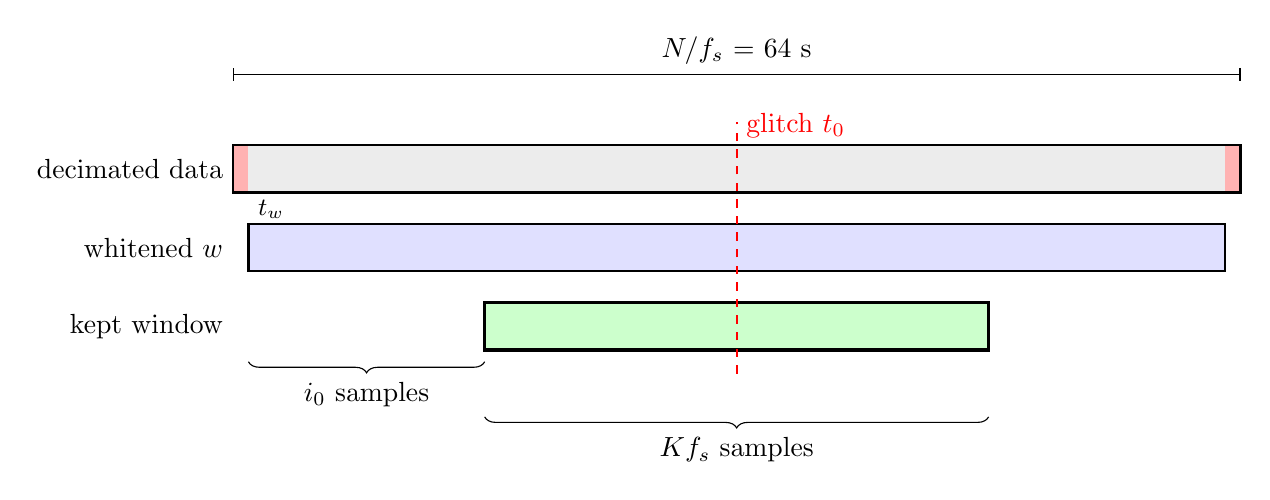
\begin{tikzpicture}[x=0.2cm, y=1cm, >=Stealth]
  % fetched data: 64 s, with the p samples the whitening corrupts at each end in red
  \draw[thick, fill=gray!15] (0,2) rectangle (64,2.6);
  \fill[red!30] (0,2) rectangle (1,2.6); \fill[red!30] (63,2) rectangle (64,2.6);
  \draw[thick] (0,2) rectangle (64,2.6);
  \node[left] at (0,2.3) {decimated data};
  % whitened: 1 s shorter at each end
  \draw[thick, fill=blue!12] (1,1) rectangle (63,1.6);
  \node[left] at (0,1.3) {whitened $w$};
  \node[above right, font=\small] at (1,1.55) {$t_w$};
  % kept window: K s centred on the glitch
  \draw[very thick, fill=green!20] (16,0) rectangle (48,0.6);
  \node[left] at (0,0.3) {kept window};
  % glitch
  \draw[dashed, red, thick] (32,-0.3) -- (32,2.9);
  \node[right, red] at (32,2.85) {glitch $t_0$};
  % lengths
  \draw[|-|] (0,3.5) -- node[above] {$N/f_s$ = 64 s} (64,3.5);
  \draw[decorate, decoration={brace, mirror, amplitude=4pt}] (1,-0.15) -- node[below=4pt] {$i_0$ samples} (16,-0.15);
  \draw[decorate, decoration={brace, mirror, amplitude=4pt}] (16,-0.85) -- node[below=4pt] {$K f_s$ samples} (48,-0.85);
\end{tikzpicture}

\smallskip
{\small Red: the $p$ samples at each end that the whitening corrupts and drops.}
\end{center}

\section*{Example}

With $f_s = 4096$~Hz, $\tau_f = 2$~s ($p = 4096$), $K = 32$~s and data starting exactly at $t_0 - 32$~s:
\[
  t_0 - t_w = 31~\text{s}, \qquad n_0 = 31 \times 4096 = 126\,976, \qquad i_0 = 126\,976 - 16 \times 4096 = 61\,440 ,
\]
which equals the earlier fixed crop, $16 \times 4096 - 4096 = 61\,440$ samples.

\section*{In the code}

\begin{lstlisting}[language=Python]
t_white0 = data.t0.value + whiten.pad / fs                       # t_w
i0 = int(round((t0 - t_white0) * fs)) - keep * fs // 2           # n_0 - K f_s / 2
if i0 < 0 or i0 + keep * fs > white_sage.numel():                # validity
    raise ValueError("the glitch is too close to the edge of the data")
white_sage = white_sage[i0:i0 + keep * fs]                       # K f_s samples
tc = t0 - (t_white0 + i0 / fs)                                   # tau_c, ~ K / 2
\end{lstlisting}

\end{document}
